\chapter{Proposed computational model}\label{chapt:model}
[\textit{By combining the power of (a) Super-resolution: EDSR, (b) D-LinkNet and taking care of noise in the intermediate step of (a) and (b), we enhance the accuracy of our deep learning model}]

\section{Super-resolution: EDSR}
Our input image does not have sufficiently high resolution to identify small roads. To solve this problem, we use the concept of super-resolution. In this proposal, we plan to use the EDSR model % \cite{EDSR}
This model is based on a modified ResNet architecture and can be used for low-level and high-level computer vision problems. The models as propsed \cite{EDSR} is shown in Figure~\ref{fig:model_EDSR}. \par

\begin{figure}[h!]
  \centering
  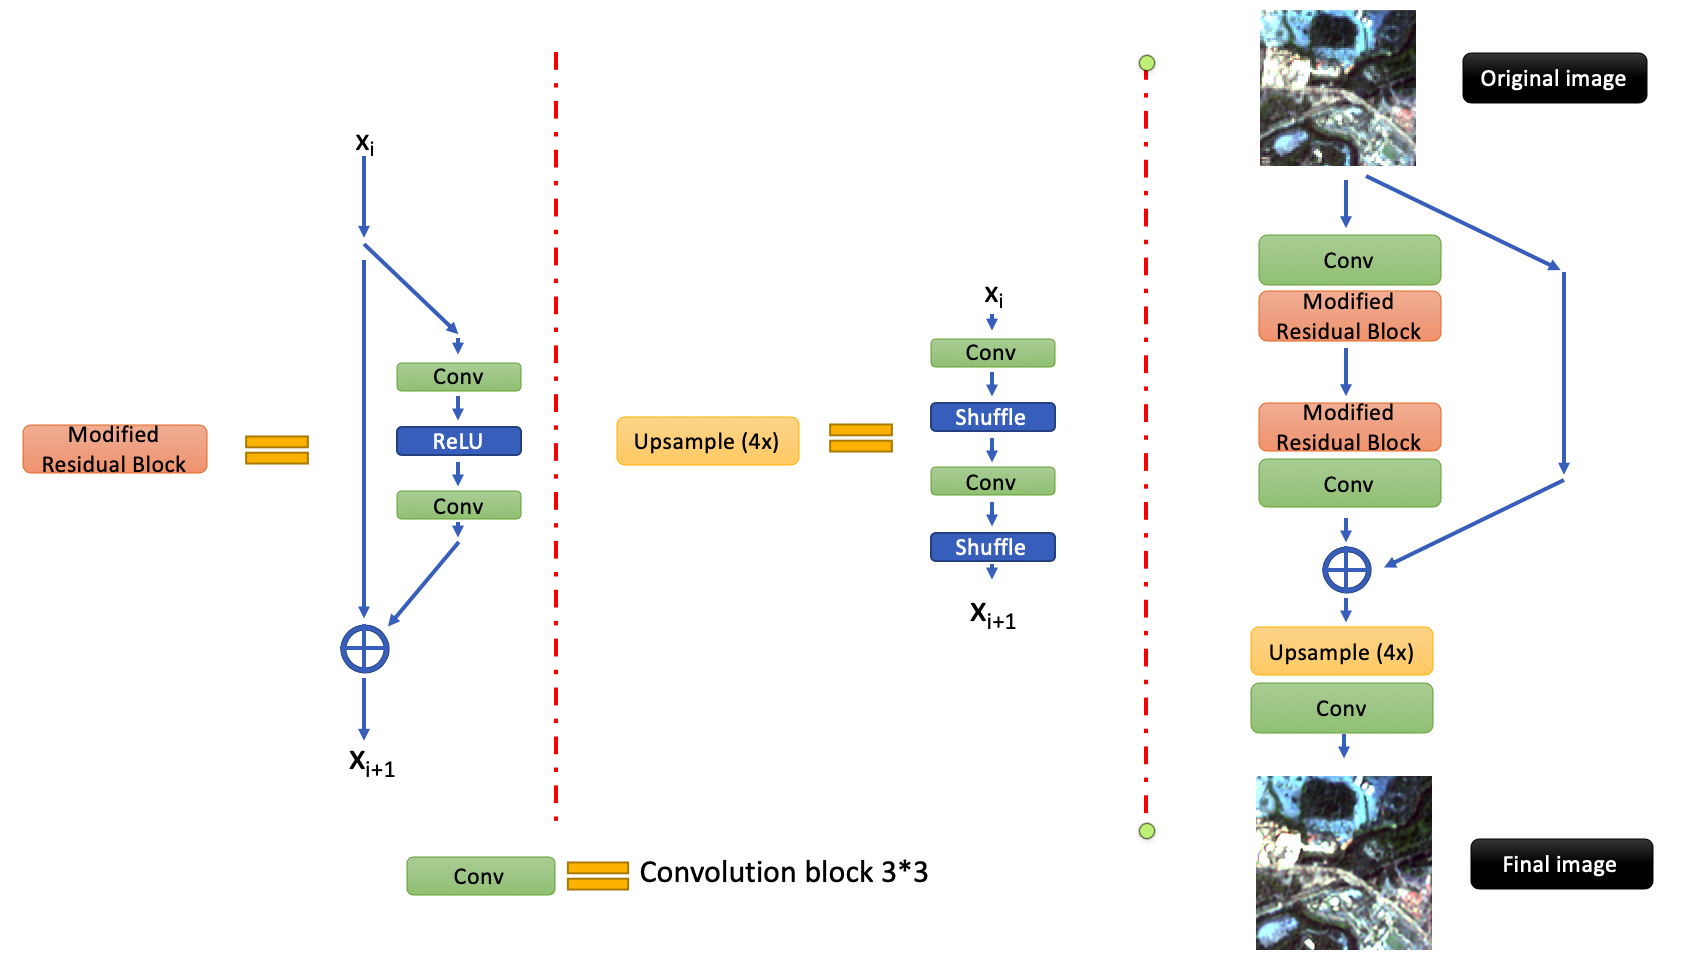
\includegraphics[width=\textwidth]{model_EDSR}
  \caption{Laying out the Strucutre for EDSR \cite{EDSR}.}
  \label{fig:model_EDSR}
\end{figure}

\section{D-LinkNet: Finding the road networks in the image}
Finding roads is a segmentation task. In D-LinkNet, the road extraction task is taken as a binary task to generate pixel-level labeling of roads. Going with deep learning models, we can classify the data by learning the weights during the training phase. However, roads are connected and spatially continuous. To take this continuity into account, we try out a fully connected network[FCN]. FCN can produce a segmentation map for an entire input image in a single forward pass. Based on FCN's, a semantic segmentation network, named D-LinkNet is propsed \cite{D-LinkNet}. \par

D-LinkNet uses an encoder-decoder architecture that accepts a single element of the input sequence, processes it, collects information from that element, and propagates it forward to the next step. This means that when the encoding is complete, the entire information is available in the intermediate step. This intermediate step is handled by using dilated convolution layers, which enlarge the receptive field of feature points without reducing the resolution of the image. Due to the complete sequence available, the decoder can make accurate predictions at each time step. \par

\begin{figure}[t]
  \centering
  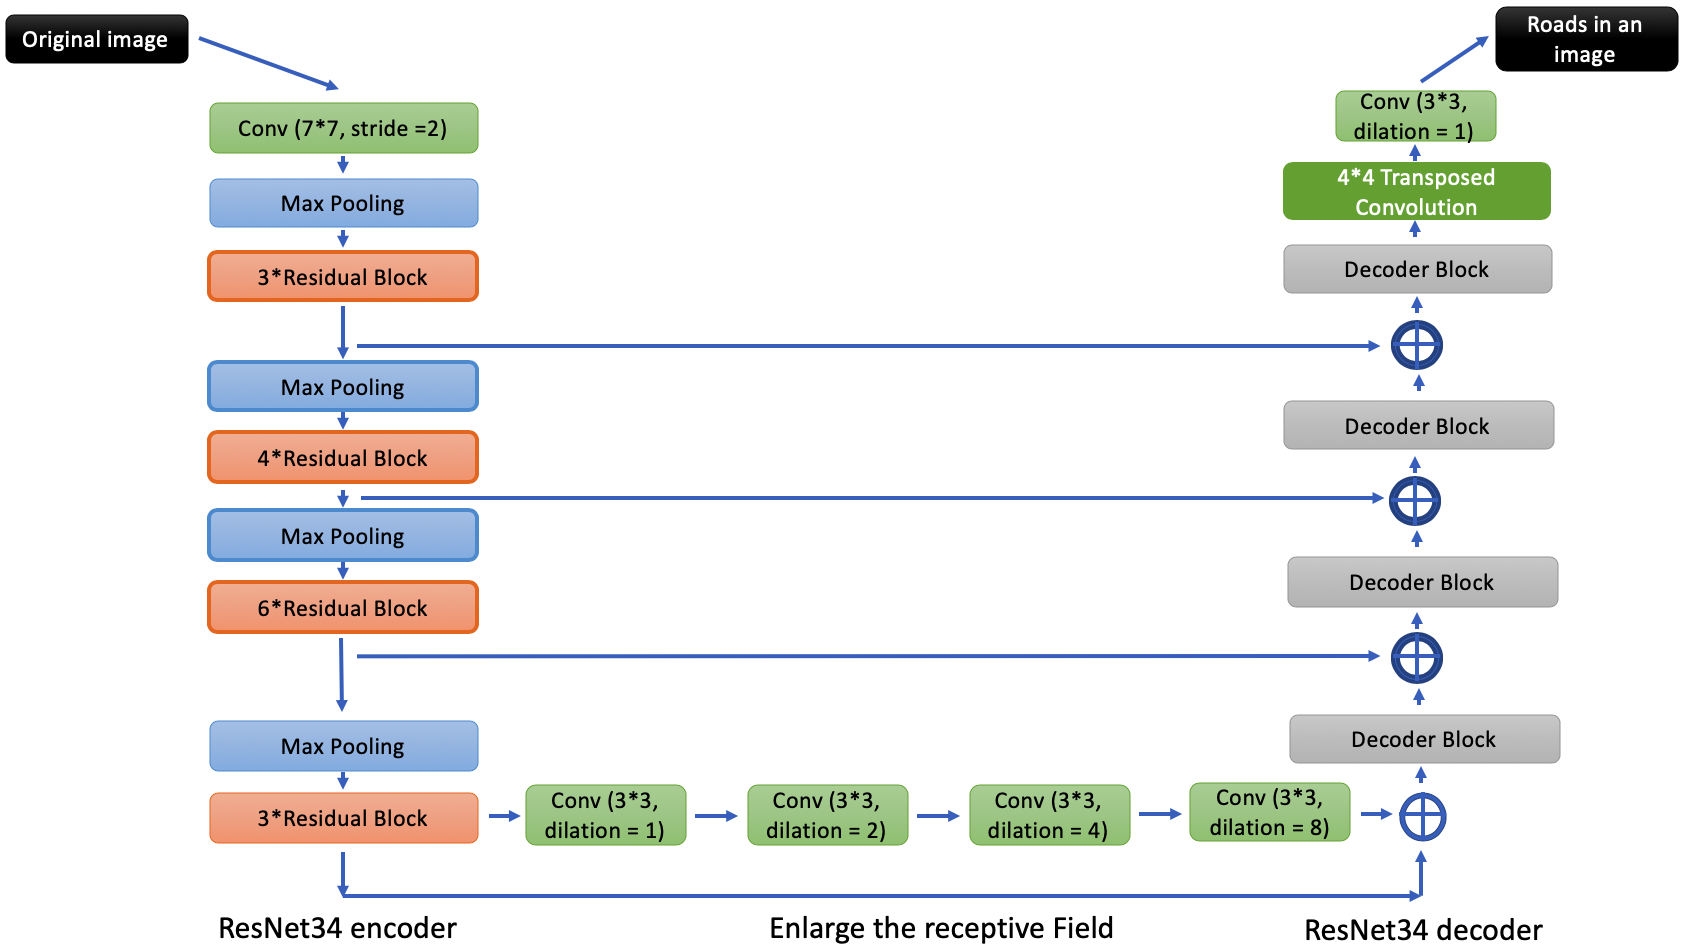
\includegraphics[width=\textwidth]{model_D-LinkNet}
  \caption{Laying out the Strucutre for D-LinkNet \cite{D-LinkNet}.}
  \label{fig:model_D-LinkNet}
\end{figure}


\section{Handling the noise generated to improve training}
Now that the models are chosen, we will now try to link the output of the super-resolution model to the input of road-detector. As specified earlier, our road-detection model assumes the training and input dataset ideally is a pixel-level accurate map. This underlying condition needs to be handled to reduce false predictions in the model. \par

The datasets constructed from a map suffers from two types of labeled noises[Figure~\ref{fig:noise_types}]:
\begin{itemize}
  \item Omission noise is when the map is incomplete. It is true for small roads and alleys.
  \item Registration noise is when the location of the object is inaccurate. This noise is quite common, as maintaining pixel-level accuracy is quite difficult to produce.
\end{itemize}

\begin{figure}
  \centering
  \begin{subfigure}{0.5\textwidth}
    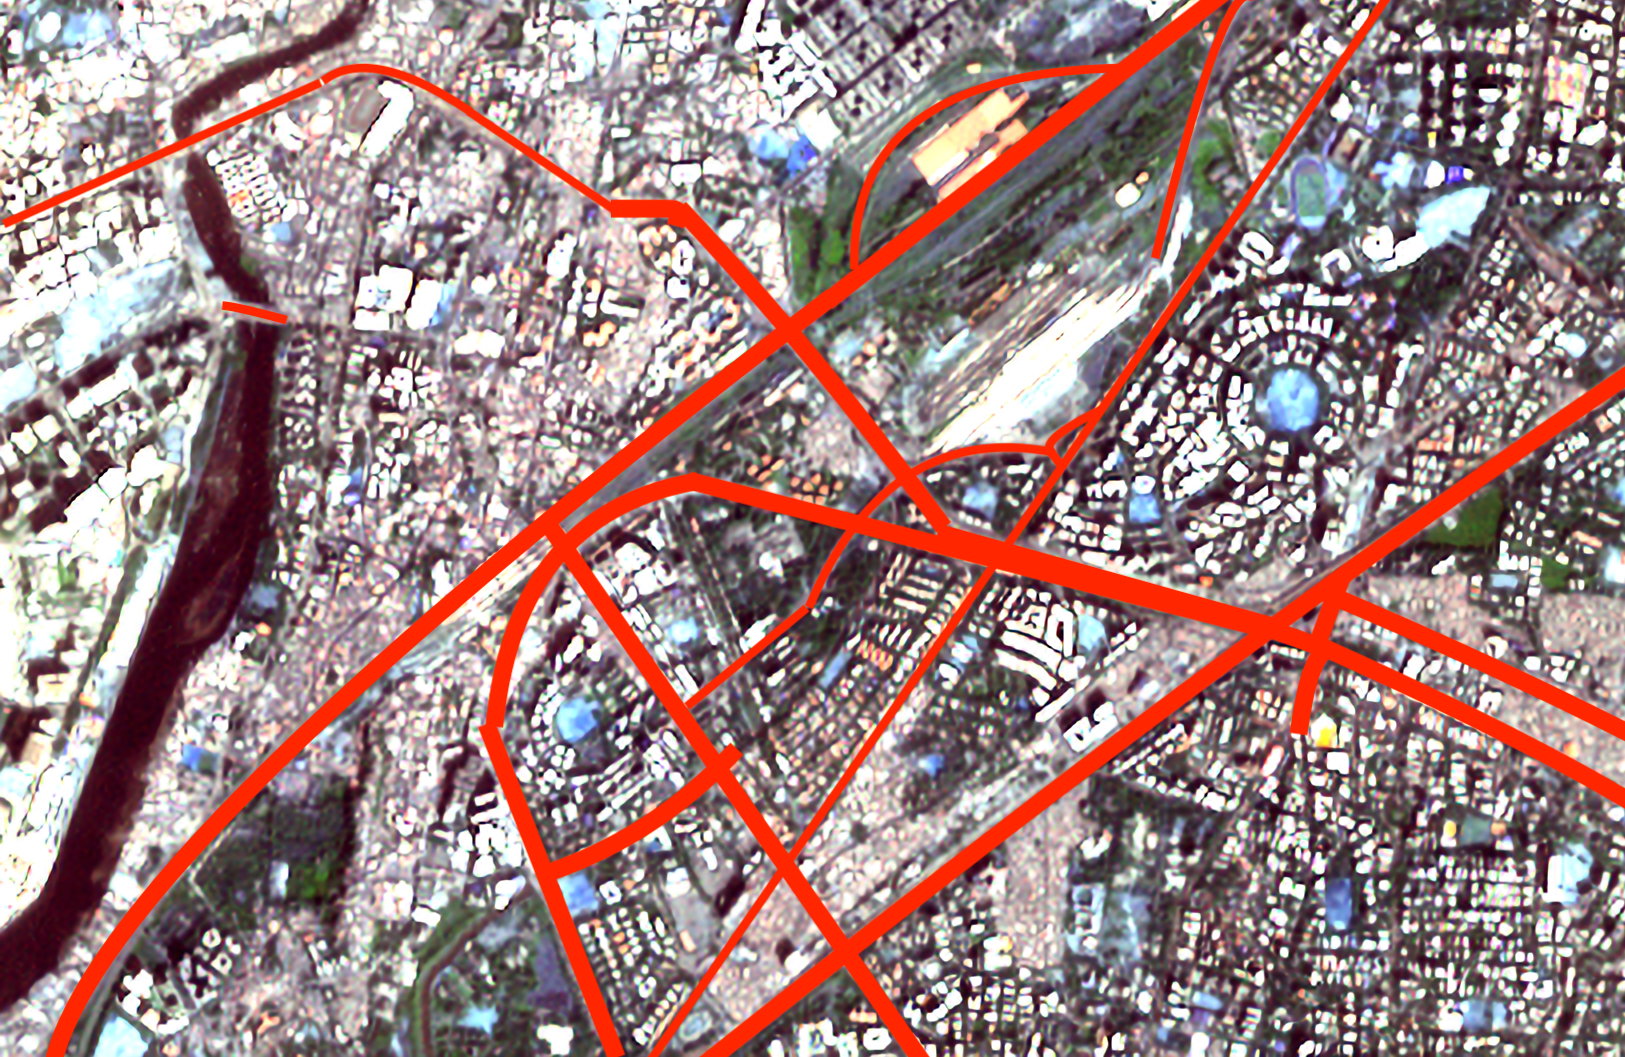
\includegraphics[width=\textwidth]{noise_omission}
    \caption{}
  \end{subfigure}~
  \begin{subfigure}{0.5\textwidth}
    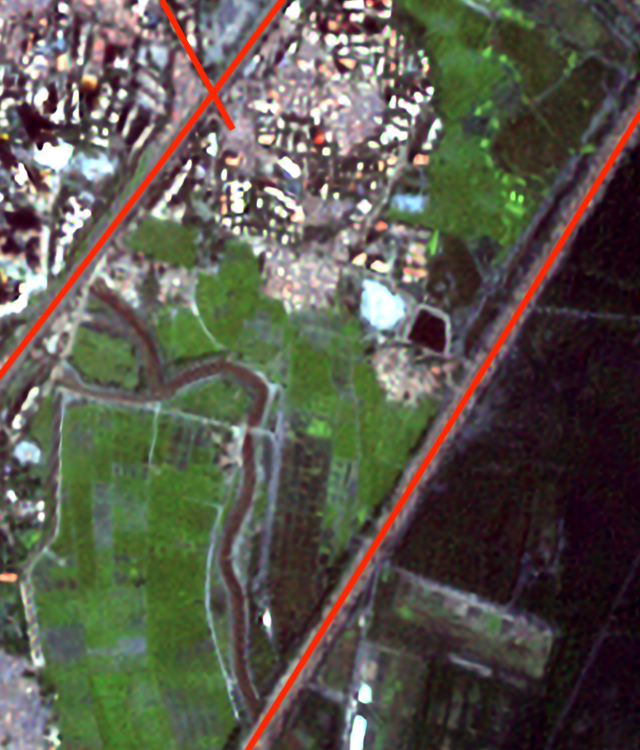
\includegraphics[width=\textwidth]{noise_registration}
    \caption{}
  \end{subfigure}
  \caption[Types of noises in a dataset]{Types of noises in a dataset (a)~Omission noise (b)~noise registration.}%
  \label{fig:noise_types}%
\end{figure}

These kinds of errors in the training labels reduce the accuracy of classifiers trained with this data. 

% \section{Applying models}
% The idea is to use super-resolution to enhance the resolution of the image and then use it to identify roads. This naturally means I take up two models: one for applying super-resolution techniques and the other for detecting roads from the images.

% Here, road segmentation is solved by generating pixel-level labeling of roads. This is done by a binary decision which we get from semantic segmentation.
